\section{Implementation} \label{implementation}
In this project, both the VM emulator and the CPU emulator were implemented. Yet, this decision to also implement the CPU emulator was made relatively late in the implementation process because it was difficult to accurately estimate the time required to implement the VM.
The CPU emulator is also much simpler than the VM and can reuse some of the code from the VM implementation.
Accordingly most of this section only focusses on the VM emulator. If no emulator is explicitly specified, the text is always referring to the VM.

\subsection{General approach}
For any project, one must first decide on a course of action. Due to the relatively unique requirements of this project, the order in which the features should be implemented is not immediately obvious.
Fundamentally, there are are two possible approaches. In a top-down approach, one would start by implementing the user interface (UI) first and then fill in the gaps later.
However, since the application has different user interfaces depending on the intended use, it makes more sense to develop bottom-up.
This allowed for a more test-driven approach, where the internal logic of the emulator is developed first and only later integrated into the UI.
In order to be able to test the VM properly, it made sense to implement the bytecode parser first~\ref{parser-dev}, as it would significantly reduce the effort required to write unit tests for the VM.
Once the parser was completed, the VM could be implemented in isolation and independent of the future user interface. The various instructions of the VM vary in complexity, so it made sense to postpone the implementation of the Function, Call and Return instructions until all other instructions had been implemented and sufficiently tested.
Here, the tests in the course projects, which were intended to test the participants' compiler implementation, helped to ensure the correct functionality of the emulator.
Although there was no way to parse the test scripts directly at this point, they were still very useful because they could easily be translated directly into rust code by hand.
Eventually all instructions were implemented according to their specification~\cite{nisan2005}.
At this point the emulator was fully functional, but the standard library was simply loaded in its bytecode form, which made it possible to execute any VM program without any modifications. The standard library would later be implemented in Rust for performance reasons~\ref{jack-stdlib-in-rust}.

% \subsubsection{Test driven development of the VM without an UI}
% \begin{itemize}
%   \item first implement bytecode parser, because it can be used in VM Tests
%   \item basic VM features (everything except for function, call, return)
%   \item testing with unit tests (Translations of VME.tst tests)
%   \item rest of the VM instructions
%   \item stdlib only as vm bytecode
% \end{itemize}

\subsection{Architectural overview}
The general architecture of the application is outlined in \cref{fig:arch}. Every box in this diagram represents a Rust module, which can either be a single file or an entire directory.
It is divided into three major sections. The actual simulators, the parsers and the interfaces that serve as entry points into the application. Even though the CPU and VM are usually refered to as emulators, the module is called simulators because that is a more general term, that would also fit the hardware simulator which was not implemented as part of this thesis~\ref{future-work}. This is the naming convention of the official tools, where the emulators are also part of the simulators package~\cite{n2tsimulators}. The two terms will therefore be used interchangeably in the following sections.

\begin{center}
  \begin{figure}[ht]
    \centering
    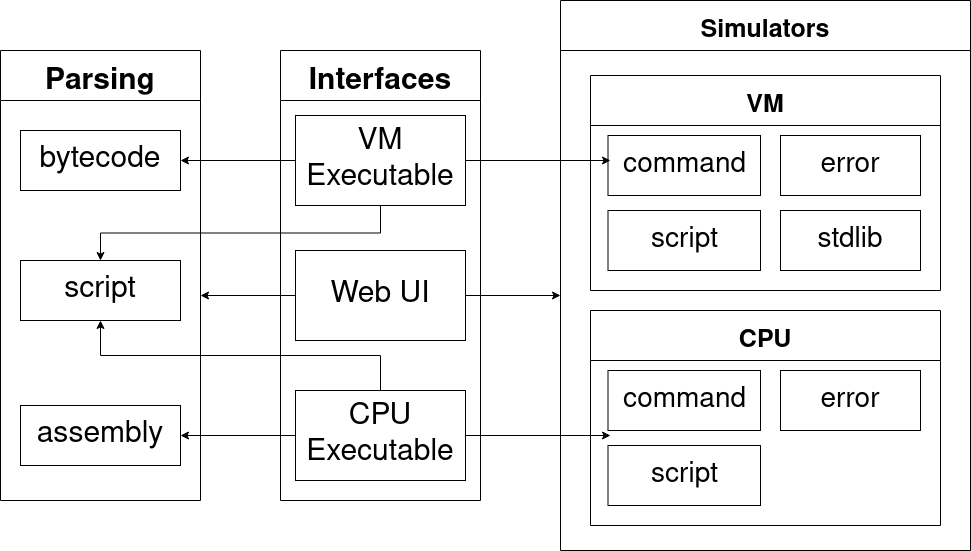
\includegraphics[width=12cm]{fig/architecture.png}
    \caption{Architecture overview diagram.}%
    \label{fig:arch}
  \end{figure}
\end{center}

\subsubsection{Interfaces} \label{interfaces}
There are three possible entry points for the application, listed in the Interfaces section of the figure. Two of them are intended for use via the command line. They provide the ability to use the test scripts included in the project within the new emulator.
They operate in slightly different ways, however, because the VM emulator can run without a test script, while the CPU emulator does not currently have this capability.
For this reason, the VM emulator expects either a path to a directory containing bytecode or a path to such a test script instead, while the CPU emulator only accepts a file path for a test script as input.
If the user passes a path to a directory, the application loads all files with the vm extension from that directory and then tries to execute them by calling the \verb+Sys.init+ function, which in turn should call the main function. If a test script is passed instead, that script is executed as described in~\cref{test-script-workflow}.
In the first case, a window is displayed if the application was compiled with the desktop function enabled. Otherwise, a message is output telling the user that the application is running in headless mode.
Other options are also available to the user, such as the ability to set the tick speed or print the output of the test script to stdout instead of writing it into the output file described in the test script.
There is also the possibility to use the bytecode implementation of the whole standard library instead of the one written in Rust.
All of the options can be listed with the ``-h'' flag.

The third entry point is the most important for most users. The Web UI, a JavaScript application that calls the emulator implementations as a WebAssembly library, is easily accessible in any standard web browser.
Unlike the other two entry points, which can only use one of the emulators at a time, the Web UI can use both simulators, indicated in the diagram by an arrow pointing to the outer simulator box. However, it does not currently support test scripts~\ref{future-work}.
This entry point can be used without the need to install additional software on the user's system by simply launching a web page in the browser. The current address of this web page is given in the readme file in the root directory of the project.


\subsubsection{Simulators and Parsers}
The two emulators in the simulators module are structurally very similar. Both have a Command module that contains the instruction enum~\ref{rust-vm-dev}, an Error module that contains the error enum for the respective emulator and a Script module that handles the emulators execution if run via a test script.
However, the VM is more complex and also contains the Stdlib module, which contains the Rust implementation of the Jack standard library~\ref{jack-stdlib-in-rust}.

Unlike the simulators module, the Parsing module actually contains three different submodules, as the script parsing is mostly independent from the emulator implementation used.
Having said that, there are some emulator specific instructions in the scripts whose parsing is actually contained in the Script module of the respective emulator. This division was done intentionally, because parsing those instructions is only a small part of the whole script parsing process and is closely linked to the way the script is interpreted by the emulator.
All of the parsers share a lot of common code, so it makes sense to combine them into one module.

\subsection{VM development in Rust} \label{rust-vm-dev}
The following sections offer a mix of general techniques for VM development in Rust, while explaining the specific choices made during the development of this project.
All processors and their emulators basically work according to the same three-stage cycle. First they fetch the next instruction to be executed. The internal number containing the current instruction is called the program counter in the following sections.
After the instruction is fetched, it is decoded, i.e., the emulator determines what type of instruction it has just fetched and, if necessary, decodes the arguments for that instruction.
The final step is the actual execution, which is of course specific to the instruction in question~\cite{nystrom2021crafting}.

\subsubsection{The internal representation of bytecode}
Before starting to implement a VM, one must first decide on an internal representation for the bytecode that will run on that VM.
The bytecode design will always involve tradeoffs between performance and ease of use during development.
The authors of the original emulator implementation chose a very inefficient representation where each instruction is an object of an instruction class. The instruction class contains a field for the opcode, the actual instruction that is executed, and several fields for possible arguments, in addition to another integer that determines the number of arguments.
On top of that, it also contains a string argument that is used for call instructions, because functions are actually called by their name at runtime.
This design has several disadvantages. From a performance perspective, it is very wasteful. Each instruction has the maximum size, even if it takes no arguments. More importantly, each instruction must be allocated on the heap and therefore requires pointer indirection during execution, which is know to have drastic impacts on performance as it reduces spatial locality~\cite{6498541}.
Furthermore, using strings to dispatch call instructions is a lot less efficient than just jumping to the correct bytecode position directly.

Two different bytecode designs were considered during the development of the new emulator.
The first, which is more efficient but also posed serious problems from an implementation point of view, uses unions to minimize the space required for storing the instruction vector~\ref{lst:original-bytecode}.
A union is similar to a struct, but only one declared field is used in a particular instance at one time~\cite{klabnik2019rust}. This allows putting opcodes, segments, and constants into a single type.
Since each of the union variants can be represented by a single byte, the entire union also fits into only a single byte. This byte can then be interpreted either as opcode, as a segment or as a constant byte, depending on the context, with a complete instruction then consisting of several instances of this union. This approach has the advantage that each instruction takes up only as much space as it actually needs, without padding bytes. The instruction vector is simply a vector of bytes that can be interpreted depending on the state of the VM.
However, this approach also has drawbacks. Reading the values requires unsafe Rust code, since there is no runtime information about the nature of each union instance contained in the type itself. More importantly, a single instruction in the textual representation of the bytecode can now correspond to multiple entries in the instruction vector, e.g.\ ``push segment 3'' would require three entries in the program vector. This means that the index of an instruction in the program at runtime is often significantly larger than the line number of the instruction in the input.
This has two major consequences. The first and less important is that additional metadata is required to determine the line number in the input from the current instruction in the runtime representation. This drastically increases the complexity needed to implement the code view in the UI.
The more important issue however is the reduction of the available address space. Jump instructions in the Hack Bytecode are absolute, not relative as for example in the JVM.
This means that by assigning multiple indices to each instruction, we would recude the number of available jump locations significantly, prohibiting us from loading bigger projects like Hackenstein~\ref{fig:hackenstein-offiziell}.
Alternatively, we could dispense with the one-to-one mapping of addresses and bytecode indices, but that would further complicate the VM implementation.
A similar problem has already been discussed in~\cref{pynand} to explain why translating bytecode to assembly is not a good solution for this project.

\begin{lstlisting}[
  language=Rust,
  label={lst:original-bytecode},
  caption={Bytecode representation based on unions},
  captionpos=b
  ]
  pub enum Segment {
    Argument,
    Local,
    // [...]
    Constant,
  }

  pub enum Instruction {
    Add,
    Sub,
    // [...]
    Function,
    Call
  }

  pub union Opcode {
    instruction: Instruction,
    segment: Segment,
    constant: u8,
  }
\end{lstlisting}

For the reasons mentioned above, the new emulator actually uses a different bytecode representation. Instead of focusing purely on performance, it is more similar to the official emulators's approach, but with the pointer indirections and some of the overhead removed.
This approach is based on Rust's enum types. Enums allow the programmer to define a type by enumerating its possible variants~\cite[Chapter~6]{klabnik2019rust}.
Unlike unions, enums contain the information to identify the content currently stored in them. Moreover, its variants can directly have different fields, which is possible with unions only by storing structs in them.
They are much more powerful than enums in C, which are simply an abstraction over a simple integer. Rust enums are closer to tagged unions in C, a combination of a union with a tag to identify the variant used.
Enums are typically used in conjunction with pattern matching, a feature that allows the programmer to compare a value against a series of patterns and then execute code based on which pattern matches~\cite[Chapter~6.2]{klabnik2019rust}.
This makes it very easy to not only identify the current instruction, but also extract all the necessary data from it~\ref{lst:bytecode-pattern-matching}.
With this approach, an entire instruction with all of its arguments is now contained in a single instance of the instruction enum~\ref{lst:enum-bytecode}.

\begin{lstlisting}[
  language=Rust,
  label={lst:enum-bytecode},
  caption={Bytecode representation based on a single enum},
  captionpos=b
  ]
  pub enum Instruction {
    Add,
    Sub,
    // [...]
    Push { segment: Segment, index: Word },
    Pop { segment: Segment, index: Word },
    Function { n_locals: Word },
    Call { function: Word, n_args: Word },
  }
\end{lstlisting}

\label{call-instruction}
The size of the enum type corresponds to the size of its largest variant in addition to a tag, so padding bytes must be added at the end of smaller variants. This may sound wasteful at first, but it is actually not a problem.
By writing a script that groups the lines of all bytecode files in a directory based on their first word, one can analyze the frequency of different instructions in VM programs.
In fact, analysis of several different Jack programs~\ref{table:tested} and the Jack standard library showed that push and pop together account for about 70\% of all bytecode instructions in real programs, while call instructions make up another 10\%.
Call instructions in the new emulator are not dispatched based on the function name. Instead, the bytecode parser already resolves the name to the index of the function within the bytecode vector~\ref{bytecode-parser}, therefore enabling the VM to simply set the program counter to that value directly.
This has the additional benefit of making the Call instruction, which would otherwise be the largest variant, the same size as the Push and Pop instructions.
Since these instructions have the same maximum size, only 20\% of instructions need padding at all.
Based on this, the padding caused by using enums is not really relevant for the memory requirements and cache efficiency of actual programs.
Pointer indirections, which are however still relevant, are also not an issue in this representation, as it contains no pointers at all.
For the above reasons, this representation is a good choice, both for performance and ease of use during development.
\cref{lst:bytecode-pattern-matching} shows how pattern matching can be used in combination with enums to implement the decoding phase of the VM cycle in a clear and concise way by directly extracting the arguments of, for example, push and function instructions and binding them to new local names.
The ``tos\_binary!'' and ``?'' will be explained in~\cref{macros} and~\cref{rust-error-handling} respectively.

\begin{lstlisting}[
  language=Rust,
  label={lst:bytecode-pattern-matching},
  caption={Using pattern matching to deconstruct the instruction data},
  captionpos=b
  ]
  match instruction {
    Add => tos_binary!(self, +),
    // [...]
    Push { segment, index } => {
      let value = self.get_value(segment, index)?;
      self.push(value)?;
    }
    // [...]
    Function { n_locals } => {
      // initialize all local variables to zero
      for _ in 0..n_locals {
        self.push(0)?;
      }
    }
  }
\end{lstlisting}

\subsubsection{Step by step execution with pattern matching} \label{step-by-step}
The architecture, with its different entry points and ways to use the emulators~\ref{fig:arch}, poses unique constraints on VM implementation. In order to satisfy all those requirements, the VM runs in a way that executes one step at a time and is able to be suspended after each of those steps. This constraint will be especially important for the interaction with native rust code in the standard library~\ref{jack-stdlib-in-rust}.
In each step, the VM first fetches the current instruction from the loaded program, then performs pattern matching to extract all the required data and finally executes the instruction.
The matching process can be seen in \cref{lst:bytecode-pattern-matching}, where the segment and index of a push instruction are extracted and then used to first load the value with another method and then push it onto the stack.
Rusts pattern matching handles the selection of the correct branch automatically.

\subsubsection{Rust macros} \label{macros}
Macros are a way of writing code that writes other code, which is known as metaprogramming~\cite[Chapter~19.5]{klabnik2019rust}.
They allow the programmer to extend the language in certain ways that would not be possible with functions alone.
One of those ways is the ability to pass language operators as arguments, which would require the creation of a closure when using functions.
Another advantage of macros is that, unlike functions, they have no runtime overhead, since the code is only inserted at the position of the caller, without an actual function call at runtime.
Those advantages can be seen in \cref{lst:binary-add-macro}, which is used in the step function for bitwise and, bitwise or, addition and subtraction. The macro gets the two values on the top of the stack, casts them to a 32 bit integer for compatibility with Java, applies the operator to them and then pushes the result onto the stack.
The operator can be passed as a simple token, instead of wrapping it into an anonymous function.
\cref{lst:bytecode-pattern-matching} shows how this macro would be called to implement the Add instruction.

\begin{lstlisting}[
  language=Rust,
  label={lst:binary-add-macro},
  caption={A macro which handles binary operators in the VM emulator},
  captionpos=b
  ]
  macro_rules! tos_binary {
    ($vm:expr, $op:tt) => {{
        let sp = $vm.mem(SP)? as Address;
        // cast up to i32 to keep compatibility with
        // the official emulator in case of an overflow
        let l = $vm.mem(sp - 2)? as i32;
        let r = $vm.mem(sp - 1)? as i32;
        $vm.set_mem(sp - 2, (l $op r) as Word)?;
        $vm.add_to_mem(SP, -1)?;
      }};
  }
\end{lstlisting}

\subsubsection{Error handling in Rust} \label{rust-error-handling}
In the code examples in the sections above, there are several lines that end with a question mark. This is a direct consequence of the way that Rust handles errors.
Rust does not support exceptions. Instead it groups errors into two major categories: recoverable and unrecoverable errors~\cite[Chapter~9]{klabnik2019rust}.
Functions that have recoverable errors, such as a file not found error, return an explicit result type that can be either an error or the expected return type.
Of course, this result type is implemented as an enum, which allows the use of pattern matching to handle errors.
One disadvantage of this approach is that so many functions return results that it would be extremely tedious to match each return value against patterns.
Conversely, Rust has constructs to further simplify the handling of recoverable errors, such as the question mark operator.
This operator can be placed after any expression that has a result type. If the expression was an error, that error is immediately returned as the return value of the entire function. On the other hand, if the expression was an actual value, that value is automatically unwrapped, allowing it to be used without further checking.
The question mark operator therefore drastically reduces the amount of code required to handle errors, making them feel more like exceptions in other languages. However, the handling of recoverable errors is still fully explicit and visible to the programmer.
Unrecoverable errors, in contrast, do not need to be visible to the programmer because, by definition, the programmer cannot handle them.
They will cause the program to abort immediately and should be used only when absolutely necessary.
This can happen either intentionally, by calling the Panic function, or as a result of unpacking a result without proper handling of the error case.
Since they are generated by the panic function, unrecoverable errors are often referred to as panics.
To provide a good user experience, none of the emulator-related code contains unrecoverable errors. The only errors of this kind are in the native interfaces to the application, for example, if the window could not be initialized in desktop mode because the application is running on a server without graphical capabilities.
The emulator specific error types are located inside the error package of each emulator module~\ref{fig:arch}.

\subsection{Parser development in Rust} \label{parser-dev}
As a multi-paradigm programming language, Rust provides both object-oriented and functional features that can be used to create parsers.
Using methods on a parser type makes it easy to group the logic that acts on the state of the parser, while anonymous functions can be used to pass conditions around easily.

Parsing usually consists of at least two stages, the first being lexical analysis, also known as tokenization.
At this stage, the individual characters of the input are grouped into tokens, which are assigned tags such as identifier, number, or symbol.
This is followed by the actual parsing stage, where the tokens are further grouped into constructs, such as arithmetic expressions or loops.
A token, in its simplest form, is a tuple of a part of the original source code called a lexeme and a tag that assigns a particular meaning to the lexeme. Some things, such as parsing integer literals from strings into actual numbers, can be done either within the lexer or, alternatively, only during the actual code generation or interpretation of the program~\cite{nystrom2021crafting}.
Neither bytecode nor assembly really has any complex constructs, since both are already flat lists of instructions.
However, the test scripts also contain more complex statements, such as repeat, which is essentially a for loop.

\subsubsection{Generic lexer}
Much of the lexical analysis code can be shared by all three parsers. At its core, a lexer only needs to consume characters as long as certain conditions are met, and then return a token containing those characters, their position in the original source code for error reporting, and the type of token that was consumed.
The generic lexer therefore offers a method ``take\_chars\_while'', which again takes a higher order predicate function as its argument. This function is evaluated for each character, starting from the current position of the lexer, until it returns false for the first time. Then all characters that evaluated true when applied to the predicate are returned as a single string with information about the token's position.
In addition, there is also a method that takes a string and returns the characters until that string appears in the source code.
\label{spans}
All lexemes extracted by the generic lexer are wrapped in a span. The span is a structure that can wrap any generic inner type with information about its position in the source code, e.g.\ the line where the element occured.
This information can later be used to improve error messages for the programmer by indicating not only what went wrong, but also where it happened.

\subsubsection{Peekable as an example for the usefulness of traits}
Each parser has its own lexer, which in turn uses the generic lexer internally.
The lexers themselves are quite simple. They simply encode the rules for each token into predicates, which are then passed to the generic lexer, and then convert the string returned by that lexer into the correct token type.
To provide a more uniform interface, these lexers also implement one of Rust's most important traits, the Iterator trait.
This interface allows the use of types within for-each loops by providing a ``next'' method that can return the next element or nothing.
This would be useful in and of itself, but Rusts powerful type system offers the ability to extend types that satisfy certain conditions by wrapping them with other types that offer even more functionality.
One such type is called Peekable. This type can be wrapped around any other type that implements the Iterator trait, allowing the user to peek at the next item without actually consuming it.
Rust calls features like this ``zero cost abstractions'' because there is no runtime overhead compared to adding the functionality directly to each lexer. It is not implemented via dynamic dispatch, but is fully resolved at compile time.
In addition, the Peekable type itself also implements the Iterator trait, so it just extends the interface without removing any functionality.
Any type that implements the Iterator trait automatically has a ``peekable'' method that returns the Iterator instance wrapped in this type.

\subsubsection{Explaining the bytecode parser} \label{bytecode-parser}
The bytecode parser is the simplest of the three parsers. As shown in~\cref{lst:hack-bytecode}, it is a flat and simple format, with simple and well-defined rules. Nevertheless, it has some complexity due to the way identifiers are resolved. Functions and labels can be referenced before they are declared. This is relevant because, as described in~\cref{call-instruction}, call instructions and labels are resolved into indices in the program vector during parsing.
To achieve this, the parsing is divided into two different steps.
First, the source code is parsed from beginning to end. The bytecode vector at this stage does not yet contain the finished instructions.
Instead, it contains instances of an enum, which can be either a fully resolved instruction or a partially constructed instruction with an identifier it is waiting for. While reading the source code, the parser keeps track of all declared functions and labels.
If such an identifier is referenced in the code, the parser tries to find it in the environment. If the identifier is already declared, the instruction is inserted into the result vector as a fully resolved instruction. However, if the instruction references an undeclared identifier, the instruction is inserted with a placeholder and another string with the name of the missing identifier.
These placeholders are then replaced with the correct indices in the second stage. Here, the parser iterates over the previous result vector and handles any instructions with placeholders.
After that, the parser performs a final check to see if there are any unresolved identifiers left. If this is the case, it returns an error, otherwise the parser is done.
One thing which has yet to be explained: If function dispatching is based on the function's index in the program's bytecode vector, how are built-in standard library functions called?
These functions actually use the highest possible indices. So if \(N\) is the largest integer that still fits into Rust's index type, and if \(n\) is the number of standard library functions, then the addresses in the range \([N - n + 1, N]\) are used to call those functions.
The exact index for each standard library function is determined before parsing, so the parser can simply replace any identifier referring to such a function with the correct index.
The connection between this index and the associated identifier can be resolved bidirectionally, so the VM can simply resolve any call with an index greater than \(N - n\) to the appropriate native function.

\subsection{The test script workflow} \label{test-script-workflow}
To allow automatic testing of student submissions, the Nand to Tetris course includes test scripts for most of its projects. These scripts are able to load programs depending on the emulator, set internal values in the emulator's memory, execute the program in a certain way, and then compare the values at specific memory addresses in the emulator with expected values loaded from a file.
This functionality is not only useful for students, but also for the instructor of the course.
test scripts share most of their functionality and syntax between all three emulators, but there are some emulator-specific features that pose a challenge to implementation.
The application must know which emulator the script is to be run in, so that only the correct instructions are parsed and executed.
Since the different emulators actually produce different executables~\ref{interfaces}, the emulator is already known, but it is not immediately obvious how to structure the code to allow only some of the possible commands to occur and be executed based on the current interface, while sharing as much code as possible.

\subsubsection{Traits as an alternative to inheritance}
In an object-oriented language, functionality like that described above would probably be implemented using abstract classes or interfaces. There might be an abstract test script parser from which the specific parsers for the VM, CPU, and hardware simulator would inherit.
The simulators could also inherit from an abstract script executor class that would implement most of the commands, leaving only the emulator-specific commands to the subclasses.
While Rust supports dynamic dispatch, it does not provide inheritance as a feature of the language.
But it does offer a powerful system of type parameters and traits to specify constraints on those types.
Methods can be implemented not only directly on types, but also conditionally if a combination of types matches certain properties.
The generic test script parser expects an emulator-specific command parser as its type parameter.
All methods of the generic parser are not actually implemented directly on this parser. Instead, they are only implemented if the combination of the generic base parser and the simulator-specific parser together implement the ScriptParser trait.
The actual implementation of the parser interface is therefore not part of the module containing the generic parser. Instead, it is implemented in the simulator-specific modules.
This process is more complicated than the object-oriented solution, but has the advantage of working without dynamic dispatch. The type parameters for the simulator-specific commands can also be used to guarantee that the emulator really expects the same commands that the parser returns.
The code is presented in a simplified version in~\cref{lst:generic-parser} and~\cref{lst:vm-parser}.
In the real program, this code is more complicated due to some details of the Rust type system that do not add to the understanding of the core principles at work, so those have been omitted.

\begin{lstlisting}[
  language=Rust,
  label={lst:generic-parser},
  caption={The generic base parser for test scripts},
  captionpos=b
  ]
  // P is the simulator specific parser
  // C is the simulator specific command
  pub struct ScriptParser<P, C> {
    // fields like the peekable lexer
    [...]
  }

  impl ScriptParser<P, C>
  where ScriptParser<P, C>: SimulatorCommandParser<C>,
  {
    [...]
  }
\end{lstlisting}

The ScriptParser implementation block only becomes relevant if there is an emulator-specific parser that implements the missing parts, as shown for the VM emulator parser in~\cref{lst:vm-parser}.
Here, the SimulatorCommandParser trait is implemented for the ScriptParser in combination with the specific VMEmulatorCommandParser, neither of which would implement the trait on their own. This implementation has to contain the missing parse function for VM specific commands.

\begin{lstlisting}[
  language=Rust,
  label={lst:vm-parser},
  caption={The VM emulator specific parser for test scripts},
  captionpos=b
  ]
  pub struct VMEmulatorCommandParser {}

  impl SimulatorCommandParser<VMEmulatorCommand>
  for ScriptParser<VMEmulatorCommandParser, VMEmulatorCommand>
  {
    [...]
  }
\end{lstlisting}

% \subsubsection{Compile time check for the combination of parser and executor}
So far we have looked at the implementation of the test script parser, but of course these scripts need to be executed to be useful.
Again, since most of the logic is shared between all the simulators, the individual emulators should only implement the commands that are unique to them and share all other code.
The trait that specifies these methods will also have a generic type parameter, just as the ``C'' parameter in~\cref{lst:generic-parser}. This ensures at compile time that the parser and executor are compatible.
Rust's powerful type inference even allows it to determine the correct script parser implementation based on the executor provided. The various interfaces can simply call the ``execute\_script'' function with one of the simulators as its argument and the compiler will automatically infer the correct parser.

\subsection{The native standard library protocol} \label{jack-stdlib-in-rust}
Theoretically, the VM could simply use the implementation of the standard library written directly in bytecode.
From a functionality point of view, this implementation is almost identical to the Java implementation in the official emulator~\ref{sys.wait-compatibility}.
The reason the official emulator still has a version of this library implemented in Java is the same reason the new emulator has a Rust version of the standard library. It is much faster.
A simple example to show the huge impact is \verb+Math.multiply+. The VM does not have a dedicated multiply instruction. Instead, it relies on a software solution within the standard library. During code generation, the compiler automatically converts any multiplication in the source code into a call to this function.
The multiplication function involves 92 lines of code with calls to \verb+Math.abs+ and a loop that executes 16 times, once for each bit in the two-byte integer. A simple multiplication therefore requires hundreds of VM ticks to execute.
In the native Rust implementation, it requires only a single tick.
Other, more complicated functions may be executed less frequently, but the performance impact here is even greater.
Providing a native implementation of these functions is therefore one of the most important possible performance improvements.
Unfortunately, it is not trivial to provide such an implementation for several reasons.

\subsubsection{The issues with native functions in the virtual machine} \label{stdlib-issues}
There are several problems with integrating native code with bytecode.
First and foremost is the fundamentally different execution model. The VM runs tick-based, executing one instruction per tick. It can therefore be easily halted after each instruction.
This is not the case with Rust code, as we cannot stop a function in the middle of execution and resume it at a later time.
It is also not possible to simply run the entire function to completion within a single VM tick. Some functions in the standard library run in an infinite loop, such as \verb+Keyboard.readLine+, which does not return until the user presses the Enter key on their keyboard.
Another difficult function is \verb+Sys.wait+, which takes a number as input and waits approximately that many milliseconds.
Targeting the web browser makes this function difficult to implement, as WebAssembly does not support multiple threads at the time of writing. \verb+Sys.wait+ cannot block the only available thread, because this would cause the entire application to become unreponsive.
The implementation is further complicated by the fact that the communication is bidirectional. The standard library may only be partially implemented natively and partially as VM bytecode. This is especially likely in Project 12, where students are expected to implement the standard library themselves in Jack.
Some functions of the standard library depend on other functions of the standard library, such as \verb+Output.printString+, which must call \verb+String.length+ to work. The call to the actual length function is important here because the internal representation of strings is not part of the specification, only the interface.
In summary, the bytecode must be able to call native Rust functions, and these native Rust functions must in turn be able to call functions implemented in bytecode. In addition, there must be a way to suspend the native functions like any other bytecode function, with the ability to resume execution at any point in the future, either based on user input, elapsed time or other conditions.
The official implementation can work around many of these problems by using multiple threads that can actually be paused and resumed based on conditions.
Since this is not possible in WebAssembly, a new way of handling native standard library functions is required.

% \begin{itemize}
%   \item step by step execution -> no waiting
%   \item vm functions can call rust functions
%   \item rust functions can call vm functions
% \end{itemize}

\subsubsection{Solving those issues with a Finite-state machine}
To solve the problems described above, the new emulator uses finite-state machines.
Finite-state machines (FSMs) are a common model in computer science with a wide range of applications. An FSM can only ever be in one of a finite number of states and can transition between these states based on conditions~\cite{sakarovitch2009elements}.
The functions in the Jack standard library do not need to be able to pause at any point in the code. Instead, there are certain points at which the function can be paused, such as by calling another function, whether a VM or a native function, or by explicitly waiting for the next tick.
This allows these functions to be represented as FSMs, where each state is a non-interruptible code block after which the function is automatically suspended. Each of these code blocks returns the next state to be executed as a return value and thus serves as a transition.
When the function finishes its execution, a special state is returned, otherwise the function continues in the state returned by the last block in the next tick of the VM.
In practice, this means that each time a native function is called in the VM, a state argument is passed in addition to the VM instance and formal parameters.
This state is actually just a 32-bit integer that is initially set to zero.
The emulator manages an internal call stack, in addition to the one that is naturally built on the global stack by the VM function call protocol.
With every function call, a new element is pushed onto this internal stack. For bytecode functions, this is useful for displaying the current call stack in the user interface, but for native functions it is very important for their functionality, since this stack entry contains the state of that function.
After a native function is suspended, which in Rust just means a normal return, its state in the stack is set to the newly returned state. Or the element is removed from the stack altogether if the special final state is returned.
Each time the VM is instructed to execute a step, it first checks if the top of the internal call stack is a built-in function that needs to be continued. If it is, it calls that function again, using the previous return value as the new state.
Continuing the function in the correct place is then as simple as putting the contents of the native function into a match statement that jumps to the correct branch based on the state argument.
In addition to the state, the native function receives the VM as a mutable reference and the formal arguments as a vector of words.
Mutable access to the VM is needed for several functions, e.g.\ drawing to the display memory to display something on the screen.

This system is powerful enough to solve all of the aforementioned problems if applied correctly, which is not trivial for every function, as can be seen in~\cref{complex-example}.
% \begin{itemize}
%   \item args passed as vector
%   \item vm is also passed mutably
%   \item state (integer, initially 0) is always passed to stdlib function
%   \item stdlib function returns either Done or next state
%   \item next time it's called with next state (if not finished)
% \end{itemize}
\subsubsection{Example: Sys.wait} \label{sys.wait-example}
\verb+Sys.wait+~\ref{lst:sys.wait} is a good example of how the state argument can be used.
Since state is just an alias for u32, a 32-bit unsigned integer, it can be used as a counter.
A special case here is the requirement that the parameter be positive, since we cannot wait for a negative time period, so an error is returned in this case.
The first time the function is called, the state is zero, so we enter the second if-statement. Here the function will terminate if the user has waited a single tick or not at all.
Normally this is not the case, so the function returns 2 as the next state.
When the emulator executes the next step, it checks its internal call stack, which contains the \verb+Sys.wait+ call with state 2 as the top element.
Therefore, instead of executing the next statement, the emulator calls the wait function again, but this time with a state of 2. This means that the function skips the first and second if-statements and returns a new state of 3 instead.
This loop then continues until the state is the same size as the first argument multiplied by 1000. When this happens, the original first argument is returned inside the special Finished state, which means that the function should be removed from the emulator's internal call stack and the next statement can finally be executed.
The multiplication by 1000 is relatively arbitrary here, since the actual duration depends on the current tick rate, which is a feature of the user interface and therefore unknown to the emulator~\ref{step-by-step}.
Theoretically, it would be better to initially set the state to the current system time and then decrement it until it reaches zero again. However, this is currently not possible because WebAssembly does not provide an API for accessing the system time~\ref{sys.wait-compatibility}.

\begin{lstlisting}[
  language=Rust,
  label={lst:sys.wait},
  caption={Implementation of the Sys.wait function},
  captionpos=b
  ]
pub fn wait(_vm: &mut VM, state: State, params: &[Word]) -> StdResult {
    if params[0] < 0 {
        return Err(StdlibError::SysWaitNegativeDuration);
    }

    let duration = params[0] as State * 1000;

    if state == 0 {
        if duration <= 1 {
            return Ok(StdlibOk::Finished(params[0]));
        }
        // 2 because one tick is already used
        return Ok(StdlibOk::ContinueInNextStep(2));
    }

    if duration > state {
        return Ok(StdlibOk::ContinueInNextStep(state + 1));
    }

    Ok(StdlibOk::Finished(params[0]))
}
\end{lstlisting}

\subsubsection{Example: Output.printString} \label{complex-example}
% or Keyboard.readLine (also shows why you can't just execute the entire native function)
\cref{lst:output.printstring} shows a more complicated function which uses the system described above. This function can be used to output an entire string to the emulator's screen. However, it does not implement the entire functionality itself, instead relying on the string module to iterate over the characters, and the output module's printChar function to print just a single character.
In theory, this function would be trivial, a simple for loop from zero to the length of the string, with only a single call to the printChar function as the loop body.
Yet it is not trivial in practice due to the limitations described in~\cref{stdlib-issues}.
Each time a function is called within a standard native library function, the latter must be stopped, since the former might be a function written in bytecode, and therefore subject to the user interface's stepwise debugger.
For example, if the native output implementation is used in combination with a string implementation in bytecode, the user might reasonably expect to step through the charAt function called by the printString function in the user interface.
This is indeed possible with this system.
Features like this necessitate the complexity of these native implementations, as they cannot be implemented with a normal for loop.
In the future, it may be possible to implement this in Rust in a more idiomatic way using the planned yield statement, however this is still a proposal at the time of writing.
Most of the logic is explained in the comments of~\cref{lst:output.printstring}, but the basic idea is simply to use the state argument both as an index for the loop and to store the length of the string. This is possible because the state type is a 32-bit integer, whereas the VM emulator uses only 16-bit integers, so the state can contain two different values.
Depending on whether the state is even or odd, we alternately call the charAt or printChar function until the counter reaches twice the length of the string.

\begin{center}
  \begin{figure}[ht]
    \centering
    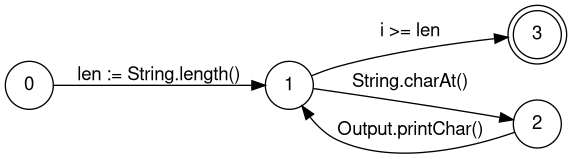
\includegraphics[width=10cm]{fig/printString.png}
    \caption{The Output.printString function as a DFA.}
    \label{fig:printstring-dfa}
  \end{figure}
\end{center}

Although the function is actually rather simple, it appears quite complicated in the code, so it is shown again in~\cref{fig:printstring-dfa}, but this time in a graphical representation of the state machine.
Each state transition in the DFA is also a suspension point for the function, with the transition to state 3 representing the final return.

\begin{lstlisting}[
  language=Rust,
  label={lst:output.printstring},
  caption={Implementation of the Output.printString function},
  captionpos=b
  ]
  pub fn print_string(vm: &mut VM, state: State, params: &[Word])
      -> StdResult {
    // State is 32 bits wide. The upper 16 bits are used to keep
    // the length information, while
    // the lower 16 bits are used for the actual state counter
    let string = params[0];
    let real_state = state & 0xFFFF;

    // in the first tick, get the length of the string to be printed
    if state == 0 {
      return call_vm!(vm, state, "String.length", &[string]);
    }

    // the second call of this function is a special case, because the
    // string length is on the stack instead of in the state
    let (len, last) = if state == 1 {
      (vm.pop()? as State, 0)
    } else {
      ((state >> 16) & 0xFFFF, vm.pop()?)
    };

    // we need 2 ticks for each i, so divide by 2
    // also subtract 1 because this will not be executed for state 0
    let i = (real_state as Word - 1) / 2;

    // the exit condition
    if i >= len {
      return Ok(Finished(0));
    }

    // keep alternating between these 2 while i < len
    if state & 1 == 1 {
      // on odd states call charAt
      vm.call("String.charAt", &[string, i])?;
      Ok(ContinueInNextStep((len << 16) | (state + 1)))
    } else {
      // on even states we actually print
      vm.call("Output.printChar", &[last])?;
      Ok(ContinueInNextStep((len << 16) | (state + 1)))
    }
  }
\end{lstlisting}

\subsection{Using conditional compilation in Rust} \label{conditional-compilation}
Like C, Rust has the ability to use macros to rewrite code at the AST level during compilation~\ref{macros}. This includes the ability to compile certain parts of the code only under certain conditions.
Not only does this feature allow features to be used only in certain builds of the application, but it also allows the programmer to specify conditional dependencies that will only be downloaded and compiled if the specific feature is enabled during compilation.
A perfect example of the usefulness of this feature is the desktop feature in the new emulator. When compiled with this feature enabled, the VM emulator can run in a native window that uses SDL2 for rendering and user interaction.
But there is no need to include SDL2 in a build that runs in the browser. So by using macros, we can compile the SDL2-related code and the library itself only when it is actually needed.
Another use case for conditional compilation is logging. Logging has a significant performance overhead if done for every command that runs in the emulator, while being rarely needed. Therefore, it is logical to hide it behind a compilation feature that can be enabled when needed and has no other drawbacks. Features are declared in the \verb+Cargo.toml+ file, which contains all project-related configuration such as the binaries built by the project, dependencies, or optimization flags.
In the code, these features can be checked with a single line of code above the block of code to be conditionally compiled~\ref{lst:conditional-compilation}.

\begin{lstlisting}[
  language=Rust,
  label={lst:conditional-compilation},
  caption={A function which is only compiled in desktop mode},
  captionpos=b
  ]
  #[cfg(feature = "desktop")]
  fn run(vm: &mut VM, steps_per_tick: usize) {
    [...]
  }
\end{lstlisting}

\subsection{Integrating the emulator into the Web UI}
So far, all sections have dealt with the internals of the emulator. However, the main goal of the project is to provide the user with a web-based interface.
Integrating the emulator into a web page is done by first compiling the Rust code into a Wasm library, which is then used by a ReactJS application~\ref{react-js}.
The exact boundary between JavaScript and Rust is arbitrary and has actually changed during the development of the application.
In the finished version, the JavaScript code requests the current frame of the screen from the Rust code, which then renders the pixel data into a JavaScript ImageData buffer, a type provided by the web-sys crate~\ref{web-sys}, and returns it. The JS code then simply displays it inside a normal canvas element.
In fact, the Rust code doesn't do anything by itself, it just provides functions that can be used by the ReactJS application.
Another example of this principle is the handling of keyboard events, which are received by JS, then passed to Rust and processed accordingly inside the emulator.
So the main loops, both for running the VM and for displaying the current frame, are written in JavaScript.
To improve performance, however, the step calls to the VM are batched.
When the emulator runs in a loop, a single iteration of the loop in the interface actually corresponds to thousands of ticks for the emulator, depending on the position of the speed slider~\ref{ui-showcase}.
Of course, this does not happen during debugging, where a single step in the user interface usually corresponds to a single tick in the emulator. The only exception to this rule is that the front-end automatically keeps ticking as long as the emulator is executing a built-in standard library function. The reason for this becomes immediately clear when one looks at~\cref{sys.wait-example}. It is not desirable to click the step button a thousand times for every second you want the emulator to wait.
By giving the front-end control over all execution, state implementation becomes much simpler, as all user interface elements can be easily updated after an event causes a change in emulator state.
If this were not the case, the emulator would have to notify the front-end of state changes, or the UI would have to actively ask the emulator for its current state as often as possible.
The interaction between the JavaScript front-end and the emulator code is facilitated by a thin compatibility layer in Rust. This layer provides a unified interface to the front-end that works for both the VM and the CPU emulators.
Therefore, there is no need to implement two different user interfaces, and all JavaScript code is shared between the two emulators.

\subsection{Web UI showcase} \label{ui-showcase}
The web based user interface is shown in~\cref{fig:ui-demo-desktop}. It is divided into four major parts.
Above everything else, there is a row with all interactive UI elements. It contains the buttons for loading a new program, starting, stopping, advancing a single step or resetting the running program and the slider for changing the VM execution speed.
In the middle left part of the screen the bytecode of the currently loaded program is displayed. This is useful when the user is using the ``Step'' button to debug the loaded program. The instruction to be executed next is highlighted in red.
To the right of that is the most important part of the user interface, the emulator screen.
Here the screen section of the emulator memory is displayed.
Below those two, certain parts of the internal memory are displayed to improve the debugging experience. From left to right, those are the call stack, local variables, arguments to the current function and the stack.
These fields are updated each time the emulator comes to a stop, i.e.\ after each step or after pressing the stop key. Since the emulator executes thousands of ticks per second, updating the values after each tick would be neither feasible nor useful, so they are only updated after stopping.
If they are not updated while running, there is no point in displaying them at all, so the bytecode view and the memory segments are hidden while the program is running. This allows the screen to fill almost the entire browser window and its contents to become as large as possible.
In contrast, the button row at the top and the screen are always visible.
\begin{center}
  \begin{figure}[ht]
    \centering
    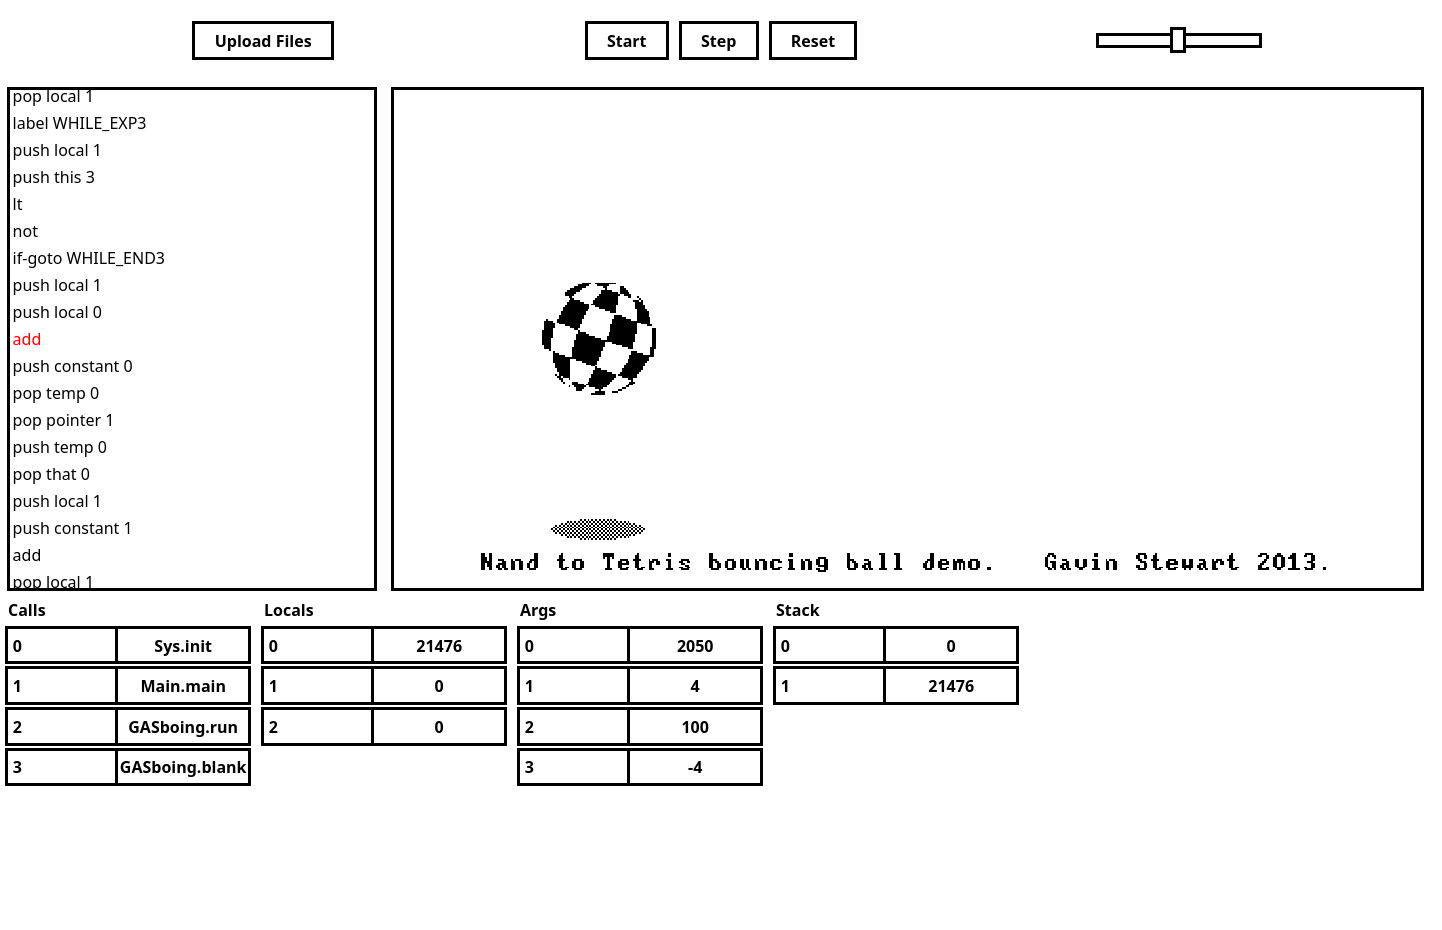
\includegraphics[width=12cm]{fig/ui-demo-desktop.png}
    \caption{The web based user interface on a desktop computer.}%
    \label{fig:ui-demo-desktop}
  \end{figure}
\end{center}
